\documentclass[11pt]{standalone}
\usepackage{amssymb}
\usepackage{amsmath}
\usepackage[no-math]{fontspec}
\usepackage{unicode-math}
\setmainfont{Libertinus Sans}
\setsansfont{Libertinus Sans}
\setmathfont{Libertinus Math}
\usepackage{pgf,xcolor}
\usepackage{tikz}
\usetikzlibrary{arrows.meta, backgrounds, calc}
\usepackage{pgfplots}
\pgfplotsset{compat=newest}
\usepackage{pifont}

\definecolor{my_darkgray}{HTML}{484949}
\definecolor{my_lightgray}{HTML}{F3F4F4}
\definecolor{my_darkblue}{HTML}{005A94}
\definecolor{my_lightblue}{HTML}{CCDEE9}
\definecolor{my_yellow}{HTML}{FFEC7F}
\definecolor{my_red}{HTML}{E60000}
\definecolor{my_orange}{HTML}{E87846}

\begin{document}
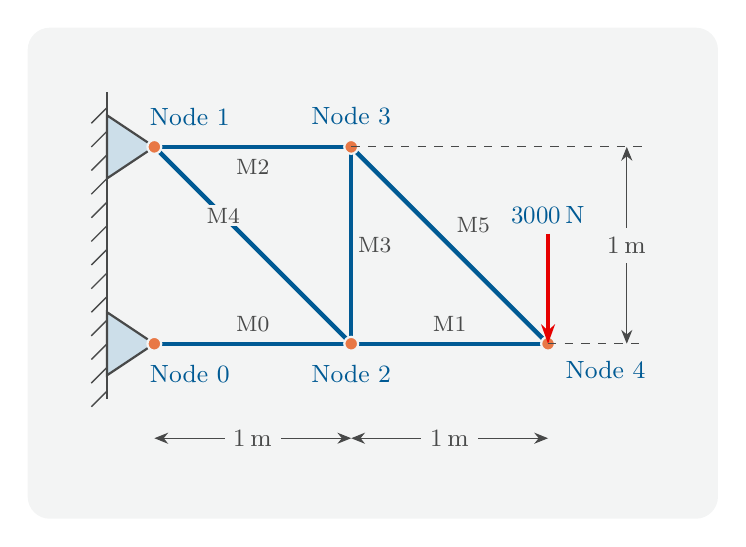
\begin{tikzpicture}[
    show background rectangle,
    background rectangle/.style={fill=my_lightgray, rounded corners=8pt},
    inner frame sep=0.8cm,
    annotation/.style={draw=my_darkgray, thick, -{Stealth[length=7pt, width=5pt]}},
    bemassung/.style={draw=my_darkgray, thin, {Stealth[length=5pt, width=4pt]}-{Stealth[length=5pt, width=4pt]}},
    stabnummer/.style={font=\footnotesize, text=my_darkgray, fill=my_lightgray, inner sep=1pt}
]

    %------------------------------------------------------------
    % Knotenkoordinaten (Faktor 2.5 gegenüber Metern):
    % Knoten 0: (0,0), Knoten 1: (0,1), Knoten 2: (1,0),
    % Knoten 3: (1,1), Knoten 4: (2,0)
    %------------------------------------------------------------
    \coordinate (N0) at (0,0);
    \coordinate (N1) at (0,2.5);
    \coordinate (N2) at (2.5,0);
    \coordinate (N3) at (2.5,2.5);
    \coordinate (N4) at (5,0);

    %------------------------------------------------------------
    % Wand mit Schraffur
    %------------------------------------------------------------
    \draw[draw=my_darkgray, thick] (-0.6,-0.7) -- (-0.6,3.2);
    \foreach \y in {-0.6,-0.3,...,3.1} {
        \draw[draw=my_darkgray, line width=0.5pt] (-0.6,\y) -- ++(-0.2,-0.2);
    }

    %------------------------------------------------------------
    % Festlager an Knoten 0 und Knoten 1 (Dreieck zur Wand hin)
    %------------------------------------------------------------
    \foreach \P in {N0, N1} {
        \draw[fill=my_lightblue, draw=my_darkgray, thick]
            (\P) -- ($(\P)+(-0.6,0.4)$) -- ($(\P)+(-0.6,-0.4)$) -- cycle;
    }

    %------------------------------------------------------------
    % Stäbe (primäres Element): my_darkblue, ultra thick
    %------------------------------------------------------------
    \draw[draw=my_darkblue, ultra thick] (N0) -- (N2);
    \draw[draw=my_darkblue, ultra thick] (N2) -- (N4);
    \draw[draw=my_darkblue, ultra thick] (N1) -- (N3);
    \draw[draw=my_darkblue, ultra thick] (N2) -- (N3);
    \draw[draw=my_darkblue, ultra thick] (N1) -- (N2);
    \draw[draw=my_darkblue, ultra thick] (N3) -- (N4);

    %------------------------------------------------------------
    % Stabnummern in der Reihenfolge der Stabliste
    %------------------------------------------------------------
    \node[stabnummer] at ($(N0)!0.5!(N2)+(0,0.25)$) {M0};
    \node[stabnummer] at ($(N2)!0.5!(N4)+(0,0.25)$) {M1};
    \node[stabnummer] at ($(N1)!0.5!(N3)+(0,-0.25)$) {M2};
    \node[stabnummer] at ($(N2)!0.5!(N3)+(0.3,0)$) {M3};
    \node[stabnummer] at ($(N1)!0.35!(N2)$) {M4};
    \node[stabnummer] at ($(N3)!0.5!(N4)+(0.3,0.25)$) {M5};

    %------------------------------------------------------------
    % Knotenpunkte (hervorgehoben): my_orange, Rand my_lightgray
    %------------------------------------------------------------
    \foreach \P in {N0, N1, N2, N3, N4} {
        \draw[fill=my_orange, draw=my_lightgray, thick] (\P) circle (2.5pt);
    }

    %------------------------------------------------------------
    % Last an Knoten 4 (3000 N nach unten)
    %------------------------------------------------------------
    \draw[draw=my_red, ultra thick, -{Stealth[length=7pt, width=5pt]}]
        ($(N4)+(0,1.4)$) -- (N4);
    \node[font=\small, text=my_darkblue, anchor=south]
        at ($(N4)+(0,1.4)$) {$3000\,\mathrm{N}$};

    %------------------------------------------------------------
    % Knotenbeschriftungen
    %------------------------------------------------------------
    \node[font=\small, text=my_darkblue, anchor=north] at ($(N0)+(0.45,-0.15)$) {Node 0};
    \node[font=\small, text=my_darkblue, anchor=south] at ($(N1)+(0.45,0.15)$) {Node 1};
    \node[font=\small, text=my_darkblue, anchor=north] at ($(N2)+(0,-0.15)$) {Node 2};
    \node[font=\small, text=my_darkblue, anchor=south] at ($(N3)+(0,0.15)$) {Node 3};
    \node[font=\small, text=my_darkblue, anchor=north west] at ($(N4)+(0.1,-0.1)$) {Node 4};

    %------------------------------------------------------------
    % Bemaßung
    %------------------------------------------------------------
    \draw[bemassung] (0,-1.2) -- node[font=\small, text=my_darkgray, fill=my_lightgray] {$1\,\mathrm{m}$} (2.5,-1.2);
    \draw[bemassung] (2.5,-1.2) -- node[font=\small, text=my_darkgray, fill=my_lightgray] {$1\,\mathrm{m}$} (5,-1.2);
    \draw[draw=my_darkgray, dashed, thin] (N3) -- (6.2,2.5);
    \draw[draw=my_darkgray, dashed, thin] (N4) -- (6.2,0);
    \draw[bemassung] (6,0) -- node[font=\small, text=my_darkgray, fill=my_lightgray] {$1\,\mathrm{m}$} (6,2.5);

\end{tikzpicture}
\end{document}
